%versi 2 (8-10-2016)
\chapter{Hasil Eksperimen di Mall Paskal 23 Square}
\label{lamp:B}

\def\scl{1}
% \def\leg{\legend{Switching,Homotopic,Buffer*Length,Length}}
\def\leg{} 
\def\std{none}
\def\ymin{}
\def\ymax{}

\section{Topologi Star}

\subsection{SensorA}
\begin{figure}[H] 
	\centering  
	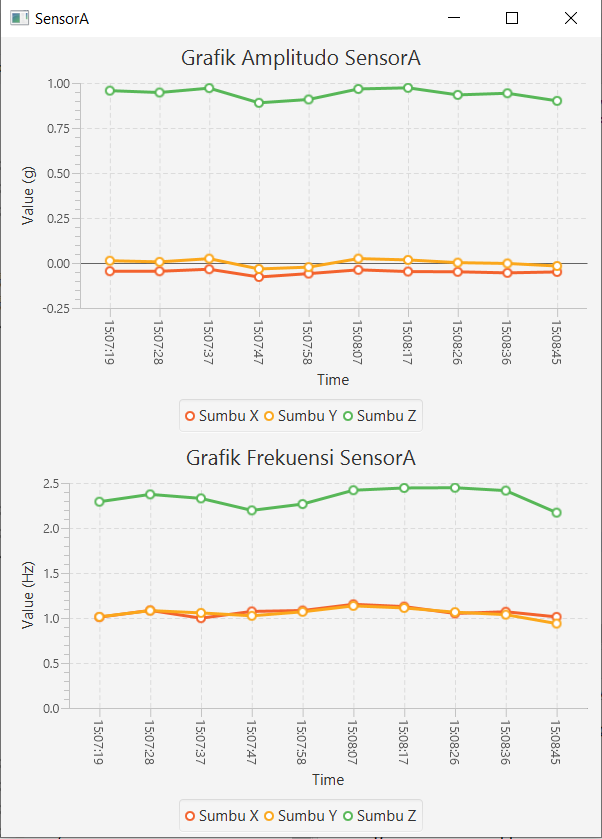
\includegraphics[scale=1]{Lampiran/HasilPengujian/sensorA_star.PNG} 
	\caption[Grafik Monitoring getaran SensorA dengan topologi star]{Grafik Monitoring getaran SensorA dengan topologi star}
	\label{fig:grafik_A_star_paskal} 
\end{figure}

\subsection{SensorB}
\begin{figure}[H] 
	\centering  
	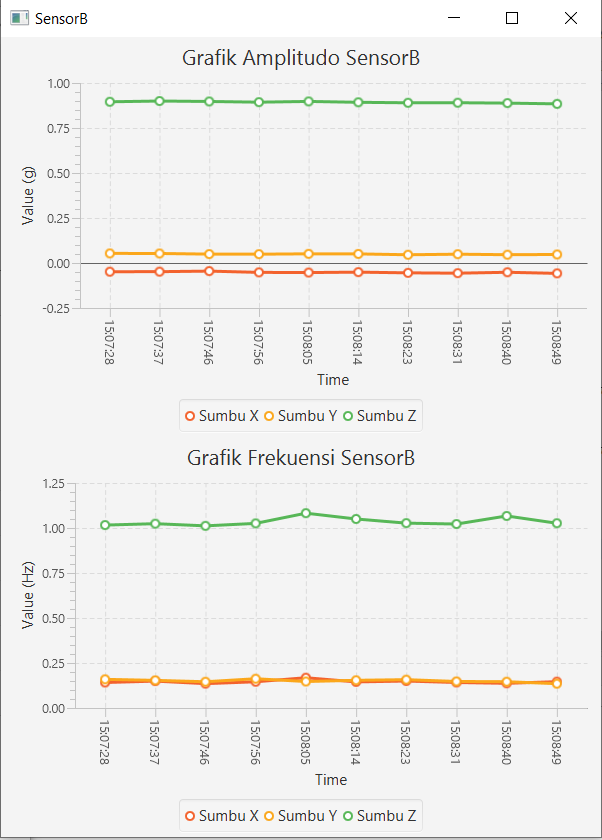
\includegraphics[scale=1]{Lampiran/HasilPengujian/sensorB_star.PNG} 
	\caption[Grafik Monitoring getaran SensorB dengan topologi star]{Grafik Monitoring getaran SensorB dengan topologi star}
	\label{fig:grafik_B_star_paskal} 
\end{figure}

\subsection{SensorC}
\begin{figure}[H] 
	\centering  
	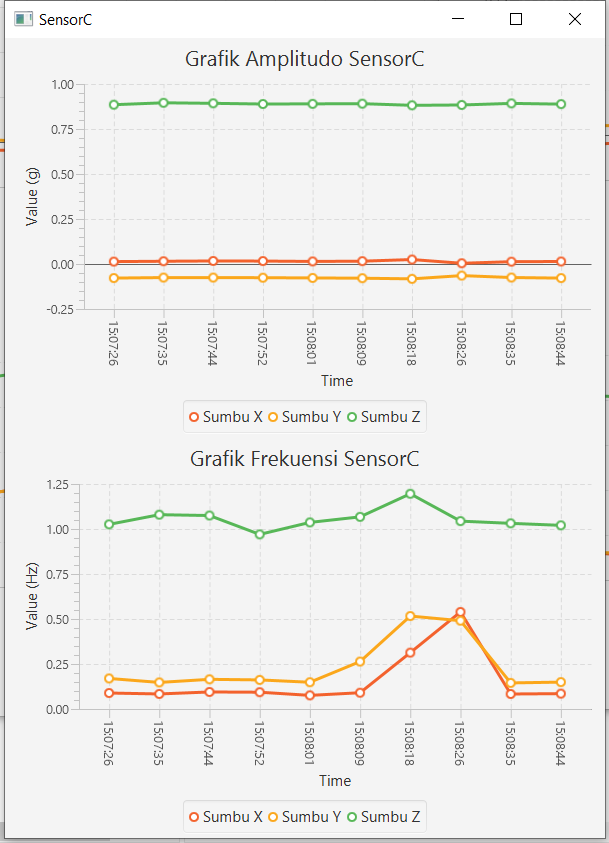
\includegraphics[scale=1]{Lampiran/HasilPengujian/sensorC_star.PNG} 
	\caption[Grafik Monitoring getaran SensorC dengan topologi star]{Grafik Monitoring getaran SensorC dengan topologi star}
	\label{fig:grafik_C_star_paskal} 
\end{figure}

\subsection{SensorD}
\begin{figure}[H] 
	\centering  
	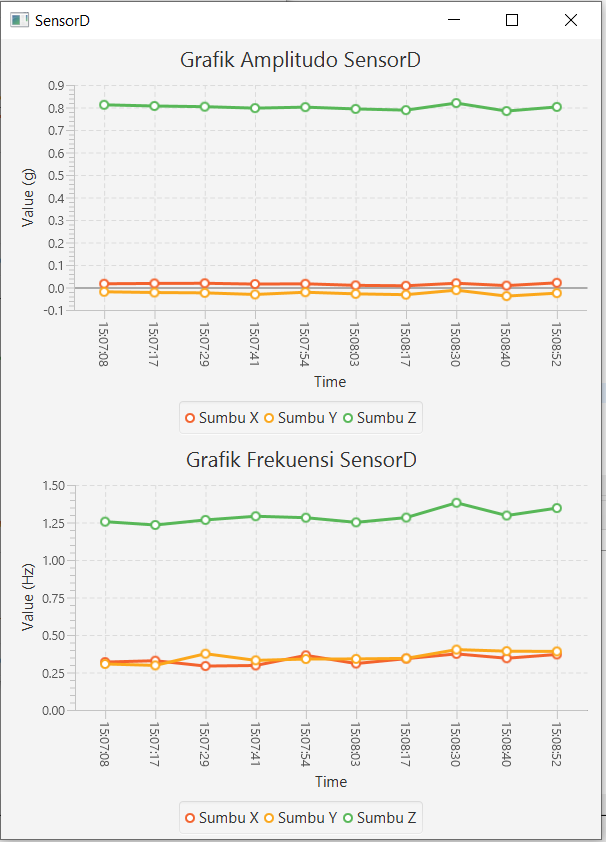
\includegraphics[scale=1]{Lampiran/HasilPengujian/sensorD_star.PNG} 
	\caption[Grafik Monitoring getaran SensorD dengan topologi star]{Grafik Monitoring getaran SensorD dengan topologi star}
	\label{fig:grafik_D_star_paskal} 
\end{figure}

\subsection{SensorE}
\begin{figure}[H] 
	\centering  
	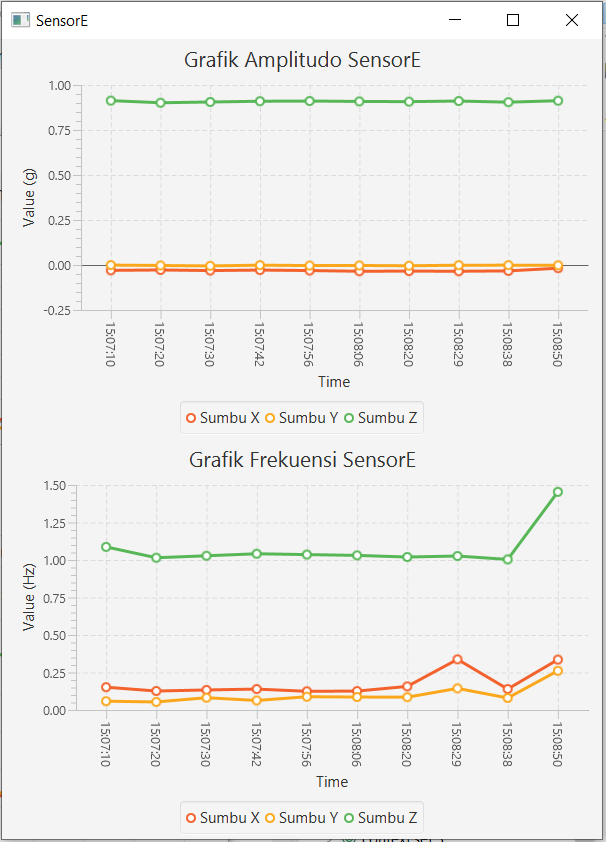
\includegraphics[scale=1]{Lampiran/HasilPengujian/sensorE_star.PNG} 
	\caption[Grafik Monitoring getaran SensorE dengan topologi star]{Grafik Monitoring getaran SensorE dengan topologi star}
	\label{fig:grafik_E_star_paskal} 
\end{figure}

\section{Topologi Tree}

\subsection{SensorA}
\begin{figure}[H] 
	\centering  
	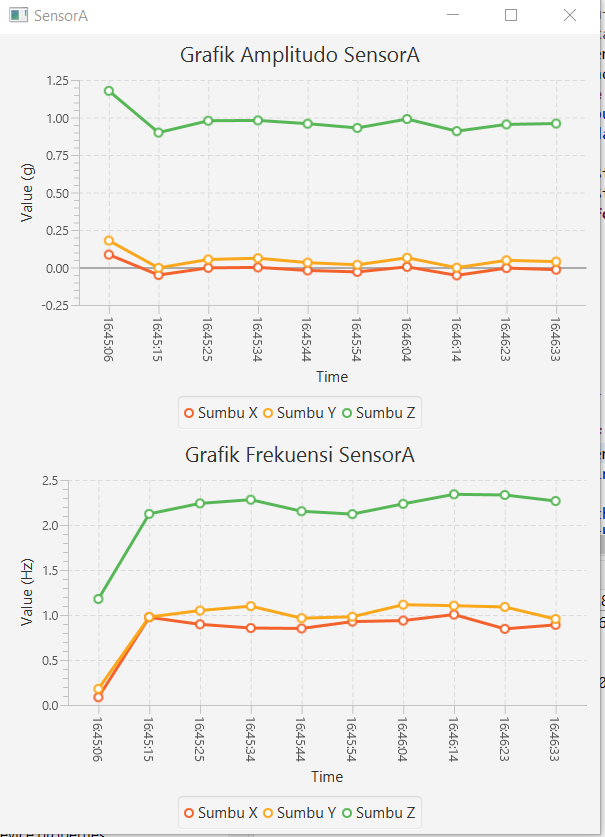
\includegraphics[scale=1]{Lampiran/HasilPengujian/sensorA_tree.PNG} 
	\caption[Grafik Monitoring getaran SensorA dengan topologi tree]{Grafik Monitoring getaran SensorA dengan topologi tree}
	\label{fig:grafik_A_tree_paskal} 
\end{figure}

\subsection{SensorB}
\begin{figure}[H] 
	\centering  
	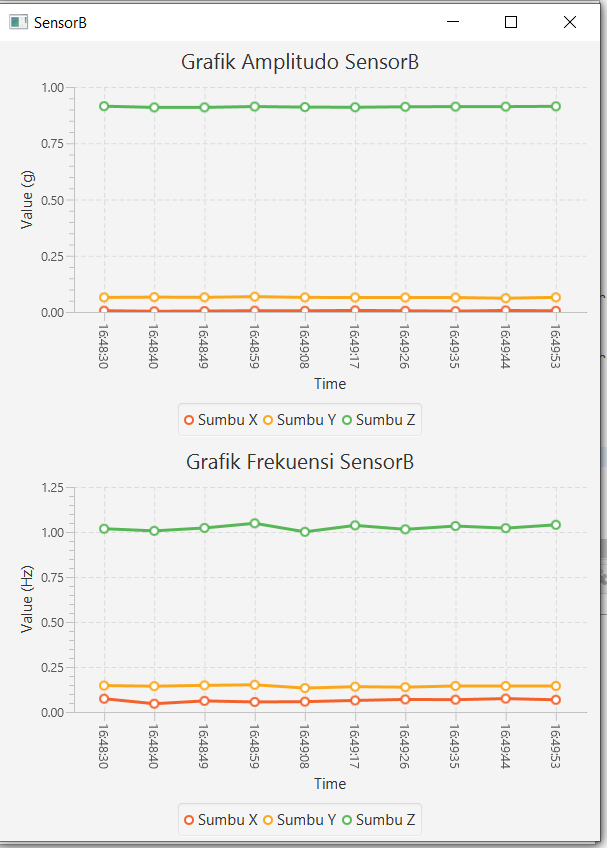
\includegraphics[scale=1]{Lampiran/HasilPengujian/sensorB_tree.PNG} 
	\caption[Grafik Monitoring getaran SensorB dengan topologi tree]{Grafik Monitoring getaran SensorB dengan topologi tree}
	\label{fig:grafik_B_tree_paskal} 
\end{figure}

\subsection{SensorC}
\begin{figure}[H] 
	\centering  
	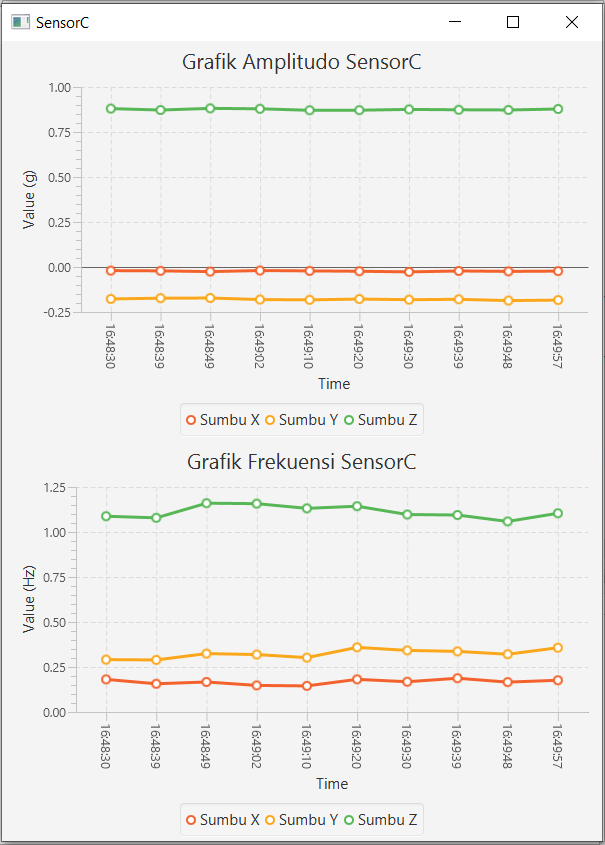
\includegraphics[scale=1]{Lampiran/HasilPengujian/sensorC_tree.PNG} 
	\caption[Grafik Monitoring getaran SensorC dengan topologi tree]{Grafik Monitoring getaran SensorC dengan topologi tree}
	\label{fig:grafik_C_tree_paskal} 
\end{figure}

\subsection{SensorD}
\begin{figure}[H] 
	\centering  
	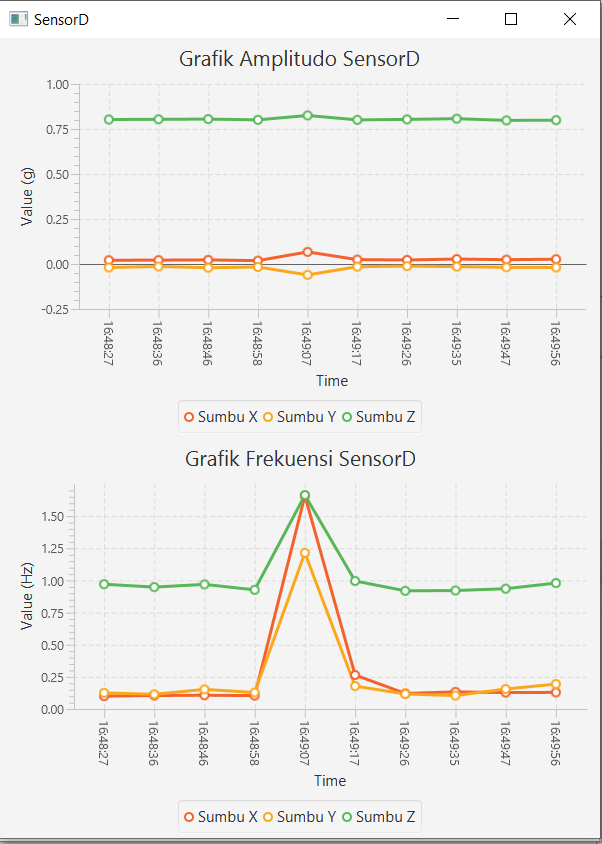
\includegraphics[scale=1]{Lampiran/HasilPengujian/sensorD_tree.PNG} 
	\caption[Grafik Monitoring getaran SensorD dengan topologi tree]{Grafik Monitoring getaran SensorD dengan topologi tree}
	\label{fig:grafik_D_tree_paskal} 
\end{figure}

\subsection{SensorE}
\begin{figure}[H] 
	\centering  
	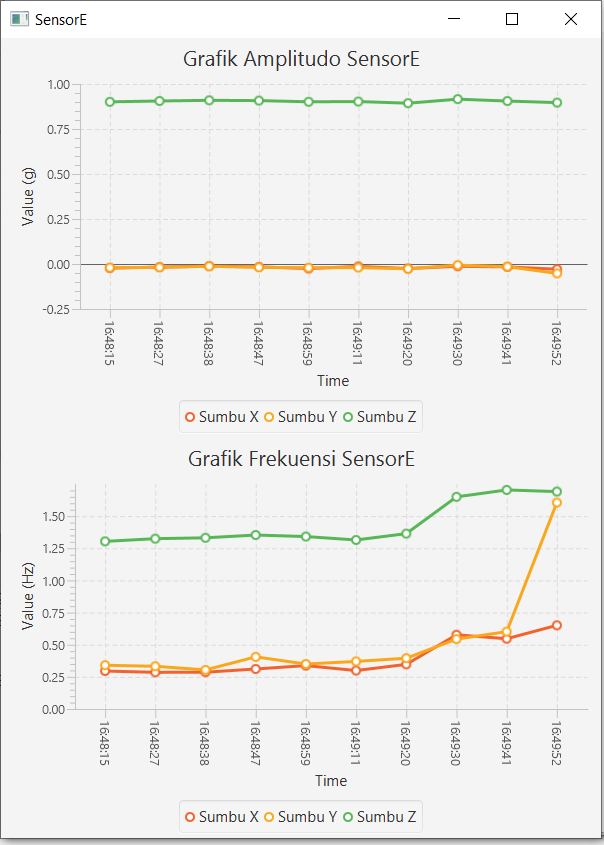
\includegraphics[scale=1]{Lampiran/HasilPengujian/sensorE_tree.PNG} 
	\caption[Grafik Monitoring getaran Sensor E dengan topologi tree]{Grafik Monitoring getaran SensorE dengan topologi tree}
	\label{fig:grafik_E_tree_paskal} 
\end{figure}